\documentclass[11pt]{article}
\usepackage[a4paper,margin=2.3cm]{geometry}
\usepackage{amsmath,amssymb}
\usepackage{booktabs,longtable,float}
\usepackage{placeins}
\usepackage{graphicx}
\usepackage[T1]{fontenc}
\usepackage{lmodern}
\usepackage{textcomp}
\usepackage{siunitx}
\DeclareSIUnit{\micrometre}{\text{\textmu}m}
\usepackage[numbers,sort&compress]{natbib}
\usepackage[hidelinks]{hyperref}
\graphicspath{{../results_v2/figures/}{../results_v2/controls/figures/}}
\renewcommand{\thetable}{S\arabic{table}}
\renewcommand{\thefigure}{S\arabic{figure}}
\renewcommand{\theequation}{S\arabic{equation}}
\renewcommand{\thesection}{S\arabic{section}}
% Generated by make_tables.py from results_v2/summary.json -- do not edit by hand
\newcommand{\EnsN}{40}
\newcommand{\MaxOcc}{0.26}
\newcommand{\LEc}{1.43}
\newcommand{\LEcCI}{1.29--1.61}
\newcommand{\LmedEc}{1.62}
\newcommand{\LminEc}{0.74}
\newcommand{\LmaxEc}{4.02}
\newcommand{\HalfEc}{1.52 and 1.37}
\newcommand{\LSa}{1.19}
\newcommand{\LSaCI}{1.08--1.33}
\newcommand{\LmedSa}{1.35}
\newcommand{\LminSa}{0.63}
\newcommand{\LmaxSa}{3.42}
\newcommand{\HalfSa}{1.24 and 1.14}
\newcommand{\LPa}{1.45}
\newcommand{\LPaCI}{1.31--1.63}
\newcommand{\LmedPa}{1.64}
\newcommand{\LminPa}{0.73}
\newcommand{\LmaxPa}{4.02}
\newcommand{\HalfPa}{1.54 and 1.38}
\newcommand{\RhoModel}{0.83}
\newcommand{\RhoModelCI}{0.81--0.84}
\newcommand{\RhoObsA}{0.70}
\newcommand{\RhoObsCIA}{0.50--0.90}
\newcommand{\RhoPctA}{89}
\newcommand{\RhoObsB}{0.91}
\newcommand{\RhoObsCIB}{0.35--1.83}
\newcommand{\RhoPctB}{40}
\newcommand{\YobsEc}{0.118}
\newcommand{\YsdEc}{0.013}
\newcommand{\LRobsEc}{0.93}
\newcommand{\SEobsEc}{0.028}
\newcommand{\LRobsBEc}{0.79}
\newcommand{\SEobsBEc}{0.16}
\newcommand{\YobsSa}{0.224}
\newcommand{\YsdSa}{0.083}
\newcommand{\LRobsSa}{0.65}
\newcommand{\SEobsSa}{0.093}
\newcommand{\LRobsBSa}{0.72}
\newcommand{\SEobsBSa}{0.22}
\newcommand{\RhoTimeMin}{0.77}
\newcommand{\RhoTimeMax}{0.80}
\newcommand{\RhoLong}{0.86}
\newcommand{\LongEcTone}{1.72}
\newcommand{\LongSaTone}{1.36}
\newcommand{\LongPaTone}{1.67}
\newcommand{\LongEcTtt}{0.96}
\newcommand{\LongSaTtt}{0.82}
\newcommand{\LongPaTtt}{0.84}
\newcommand{\LongEcTsevtwo}{0.74}
\newcommand{\LongSaTsevtwo}{0.64}
\newcommand{\LongPaTsevtwo}{0.63}
\newcommand{\RhoPPmed}{0.74}
\newcommand{\RhoPPlo}{0.69}
\newcommand{\RhoPPhi}{0.81}
\newcommand{\RhoPPorder}{100}
\newcommand{\PaGeEc}{72}
\newcommand{\PPsnakeEc}{0.84--1.97}
\newcommand{\PPsharkEc}{1.26--1.85}
\newcommand{\PPsnakeSa}{0.62--1.52}
\newcommand{\PPsharkSa}{0.94--1.40}
\newcommand{\PPsnakePa}{0.85--1.96}
\newcommand{\PPsharkPa}{1.28--1.91}
\newcommand{\PredPaMechCI}{0.87--1.00}
\newcommand{\SharkMoreMin}{85}
\newcommand{\SharkMoreMax}{91}
\newcommand{\SharkBelowSnake}{12}
\newcommand{\Alpha}{0.64}
\newcommand{\AlphaCI}{0.56--0.72}
\newcommand{\PredPa}{0.93}
\newcommand{\PredPaCI}{0.88--0.99}
\newcommand{\PredPaRem}{0.117}
\newcommand{\PredPaRemCI}{0.103--0.133}
\newcommand{\PredPaPct}{88}
\newcommand{\LosoSa}{0.77}
\newcommand{\LosoSaCI}{0.58--0.95}
\newcommand{\LosoSaPct}{12}
\newcommand{\LosoEc}{0.79}
\newcommand{\LosoEcCI}{0.56--1.01}
\newcommand{\LosoEcPct}{89}
\newcommand{\AlphaB}{0.57}
\newcommand{\AlphaCIB}{0.37--0.77}
\newcommand{\PredPaB}{0.83}
\newcommand{\PredPaCIB}{0.55--1.09}
\newcommand{\PredPaRemB}{0.149}
\newcommand{\PredPaRemCIB}{0.081--0.284}
\newcommand{\PredPaPctB}{85}
\newcommand{\LosoSaB}{0.66}
\newcommand{\LosoSaCIB}{0.14--1.17}
\newcommand{\LosoSaPctB}{61}
\newcommand{\LosoEcB}{0.87}
\newcommand{\LosoEcCIB}{0.24--1.47}
\newcommand{\LosoEcPctB}{40}
\newcommand{\SharkEc}{1.72}
\newcommand{\SharkLateEc}{1.53}
\newcommand{\SharkAlphaEc}{0.98}
\newcommand{\SharkObsEc}{2.30}
\newcommand{\SharkSa}{1.40}
\newcommand{\SharkLateSa}{1.29}
\newcommand{\SharkAlphaSa}{0.82}
\newcommand{\SharkObsSa}{1.11--2.11}
\newcommand{\SharkPa}{1.81}
\newcommand{\SharkLatePa}{1.58}
\newcommand{\SharkAlphaPa}{1.01}
\newcommand{\SharkObsPa}{1.36--3.00}
\newcommand{\NumMean}{0.028}
\newcommand{\NumMax}{0.06}
\newcommand{\NumRel}{3}
\newcommand{\NumCoarse}{0.27}
\newcommand{\NumScreen}{0.14}
\newcommand{\NumTime}{0.0015}
\newcommand{\NumDomTwo}{0.02}
\newcommand{\NumDomFour}{0.06}
\newcommand{\NumShark}{0.15}
\newcommand{\KOTrEc}{0.62}
\newcommand{\KOTrEcCI}{0.53--0.73}
\newcommand{\KOTrSa}{0.30}
\newcommand{\KOTrSaCI}{0.24--0.37}
\newcommand{\KOTrPa}{0.67}
\newcommand{\KOTrPaCI}{0.58--0.78}
\newcommand{\KOSlEc}{0.12}
\newcommand{\KOSlEcCI}{0.09--0.15}
\newcommand{\KOSlSa}{0.08}
\newcommand{\KOSlSaCI}{0.06--0.11}
\newcommand{\KOSlPa}{0.13}
\newcommand{\KOSlPaCI}{0.10--0.16}
\newcommand{\KOApEc}{\ensuremath{-}0.04}
\newcommand{\KOApEcCI}{\ensuremath{-}0.05 to \ensuremath{-}0.03}
\newcommand{\KOApSa}{\ensuremath{-}0.01}
\newcommand{\KOApSaCI}{\ensuremath{-}0.01 to \ensuremath{-}0.01}
\newcommand{\KOApPa}{\ensuremath{-}0.05}
\newcommand{\KOApPaCI}{\ensuremath{-}0.06 to \ensuremath{-}0.03}
\newcommand{\KOCoEc}{\ensuremath{-}0.17}
\newcommand{\KOCoEcCI}{\ensuremath{-}0.20 to \ensuremath{-}0.14}
\newcommand{\KOCoSa}{\ensuremath{-}0.11}
\newcommand{\KOCoSaCI}{\ensuremath{-}0.13 to \ensuremath{-}0.09}
\newcommand{\KOCoPa}{\ensuremath{-}0.16}
\newcommand{\KOCoPaCI}{\ensuremath{-}0.18 to \ensuremath{-}0.13}
\newcommand{\KOEpsEc}{0.01}
\newcommand{\KOEpsEcCI}{0.01--0.02}
\newcommand{\KOEpsSa}{0.01}
\newcommand{\KOEpsSaCI}{0.01--0.01}
\newcommand{\KOEpsPa}{0.01}
\newcommand{\KOEpsPaCI}{0.01--0.02}
\newcommand{\KOStEc}{0.01}
\newcommand{\KOStEcCI}{0.00--0.01}
\newcommand{\KOStSa}{0.00}
\newcommand{\KOStSaCI}{0.00--0.00}
\newcommand{\KOStPa}{0.01}
\newcommand{\KOStPaCI}{0.00--0.01}
\newcommand{\DesSeedSD}{0.009}
\newcommand{\DesMinEc}{0.82}
\newcommand{\DesMaxEc}{2.71}
\newcommand{\DesLowTipEc}{0.89}
\newcommand{\DesHighTipEc}{1.54}
\newcommand{\DesNarrowEc}{1.03}
\newcommand{\DesWideEc}{1.83}
\newcommand{\DesCloseEc}{2.68}
\newcommand{\DesFarEc}{0.74}
\newcommand{\DesMinSa}{0.65}
\newcommand{\DesMaxSa}{2.09}
\newcommand{\DesLowTipSa}{0.70}
\newcommand{\DesHighTipSa}{1.10}
\newcommand{\DesNarrowSa}{0.76}
\newcommand{\DesWideSa}{1.46}
\newcommand{\DesCloseSa}{2.16}
\newcommand{\DesFarSa}{0.59}
\newcommand{\DesMinPa}{0.80}
\newcommand{\DesMaxPa}{2.74}
\newcommand{\DesLowTipPa}{0.86}
\newcommand{\DesHighTipPa}{1.59}
\newcommand{\DesNarrowPa}{1.04}
\newcommand{\DesWidePa}{1.81}
\newcommand{\DesClosePa}{2.62}
\newcommand{\DesFarPa}{0.75}
\newcommand{\STPf}{0.02--0.03}
\newcommand{\STPa}{0.77--0.82}
\newcommand{\STLen}{0.01}
\newcommand{\STBw}{0.07--0.08}
\newcommand{\STTap}{0.02}
\newcommand{\STTh}{0.18--0.22}
\newcommand{\STPitA}{0.00}
\newcommand{\STPitB}{0.00--0.01}
\newcommand{\STPitD}{0.03--0.05}
\newcommand{\STJit}{0.00--0.01}
\newcommand{\STRough}{0.03--0.04}
\newcommand{\STMinor}{0.05}
\newcommand{\KOCoMin}{0.11}
\newcommand{\KOCoMax}{0.17}
\newcommand{\KOApMax}{0.05}
\newcommand{\KOSlMin}{0.08}
\newcommand{\KOSlMax}{0.13}
\newcommand{\SMBeta}{0.30--0.31}
\newcommand{\SMcBeta}{0.06}
\newcommand{\SMAdh}{0.16--0.23}
\newcommand{\SMcAdh}{0.24}
\newcommand{\SMRng}{0.14--0.20}
\newcommand{\SMcRng}{0.17}
\newcommand{\SMTrp}{0.05--0.17}
\newcommand{\SMcTrp}{0.51}
\newcommand{\SMApp}{0.00--0.00}
\newcommand{\SMcApp}{0.00}
\newcommand{\SMAnc}{0.04--0.05}
\newcommand{\SMcAnc}{0.00}
\newcommand{\SMEpsK}{0.00--0.00}
\newcommand{\SMcEpsK}{0.00}
\newcommand{\TmT}{40}
\newcommand{\TmPa}{0.81}
\newcommand{\TmSa}{0.79}
\newcommand{\ChemLowEc}{0.27}
\newcommand{\ChemHighEc}{0.02}
\newcommand{\ChemLowSa}{0.35}
\newcommand{\ChemHighSa}{0.07}
\newcommand{\ChemLowPa}{0.23}
\newcommand{\ChemHighPa}{0.01}

\newcommand{\ArrDualEc}{1.43}
\newcommand{\ArrDualSa}{1.19}
\newcommand{\ArrDualPa}{1.45}
\newcommand{\ArrDualRatio}{0.83}
\newcommand{\ArrSupplyEc}{1.24}
\newcommand{\ArrSupplySa}{1.09}
\newcommand{\ArrSupplyPa}{1.23}
\newcommand{\ArrSupplyRatio}{0.88}
\newcommand{\ArrCaptureEc}{1.16}
\newcommand{\ArrCaptureSa}{1.06}
\newcommand{\ArrCapturePa}{1.14}
\newcommand{\ArrCaptureRatio}{0.91}
\newcommand{\SpcDualEc}{1.94}
\newcommand{\SpcDualSa}{1.69}
\newcommand{\SpcDualPa}{1.89}
\newcommand{\SpcSupplyEc}{1.56}
\newcommand{\SpcSupplySa}{1.44}
\newcommand{\SpcSupplyPa}{1.49}
\newcommand{\SpcCaptureEc}{1.50}
\newcommand{\SpcCaptureSa}{1.40}
\newcommand{\SpcCapturePa}{1.43}
\newcommand{\SpcPos}{36}
\newcommand{\SpcN}{36}
\newcommand{\IndN}{160}
\newcommand{\IndOrd}{148}
\newcommand{\IndOrdPct}{92.5}
\newcommand{\IndRatio}{0.55--1.02}
\newcommand{\IndPa}{0.66--1.06}
\newcommand{\GeomMaxCovErr}{0.0001}
\newcommand{\GeomNposCoverage}{144}
\newcommand{\GeomNtotalCoverage}{144}
\newcommand{\GeomEcCovPit}{0.71}
\newcommand{\GeomEcCovNoPit}{0.48}
\newcommand{\GeomSaCovPit}{0.59}
\newcommand{\GeomSaCovNoPit}{0.53}
\newcommand{\GeomPaCovPit}{0.68}
\newcommand{\GeomPaCovNoPit}{0.43}
\newcommand{\GeomFactEc}{0.80}
\newcommand{\GeomFactSa}{0.66}
\newcommand{\GeomFactPa}{0.78}
\newcommand{\GeomFactEcLow}{0.39}
\newcommand{\GeomFactEcHigh}{1.22}
\newcommand{\GeomFactEcMin}{0.18}
\newcommand{\GeomFactEcMax}{2.49}
\newcommand{\GeomFactPos}{144}
\newcommand{\GeomFactN}{144}
\newcommand{\GeomPhaseMaxMean}{0.0013}
\newcommand{\GeomPhaseMaxAbs}{0.011}
\newcommand{\GeomGridMax}{0.148}
\newcommand{\GeomGridShort}{0.037}
\newcommand{\GeomGridWide}{0.012}
\newcommand{\GeomExtremeMaxAdditional}{0.183}
\newcommand{\GeomFinePos}{24}
\newcommand{\GeomFineN}{24}
\newcommand{\GeomFineMaxDeltaError}{0.056}

\newcommand{\TITLE}{Lateral blade packing predicts bacterial retention on reconstructed ball python scales}

\newcommand{\Ec}{\textit{E.~coli}}
\newcommand{\Sa}{\textit{S.~aureus}}
\newcommand{\Pa}{\textit{P.~aeruginosa}}

\title{Electronic supplementary material for\\[4pt]\large \TITLE}
\author{Bianca Cruz Neves and Antonio Pereira}
\date{}

\begin{document}
\maketitle

\section{Model specification}

\subsection{Blade arrays}
Blades point along $+x$ and sit on a staggered lattice in a doubly periodic cell. Following tips are $p_f$ apart along the blade axis; adjacent columns are offset by $p_f/2$ along the axis and by $p_\perp=\sqrt{p_a^2-(p_f/2)^2}$ across it, so that $p_a$ is the distance between adjacent tips. The cell contains $n_x=\max(4,\mathrm{round}(36/p_f))$ blades along the axis and an even number $n_y$ of columns close to $36/p_\perp$; its sides are rounded to whole grid steps, which changes the following and adjacent-column spacings by at most $\Delta x/(2n_x)$ and $\Delta x/(2n_y)$, respectively. Blade $(i,j)$ has its base at
\begin{equation}
\mathbf b_{ij}=\big((i+\tfrac12[j\bmod2])\,L_x/n_x+\xi_x,\;(j+\tfrac12)\,L_y/n_y+\xi_y\big),\qquad \xi_x,\xi_y\sim\mathcal N(0,\sigma_j^2),
\end{equation}
and every random attribute of the blade is drawn from a generator seeded by the triple (lattice seed, $i$, $j$), so that a blade is identical on every grid. With $u\in[0,\ell_{ij}]$ the distance downstream of the base (modulo $L_x$) and $v$ the minimum-image lateral offset, the blade occupies $|v|\le\tfrac12w_{ij}(1-u/\ell_{ij})^{q}$ and its upper surface rises linearly from the scale sheet to the tip,
\begin{equation}
z_{ij}(u)=h_{ij}\,u/\ell_{ij},
\end{equation}
with $\ell_{ij}=\ell(1+0.05\zeta_1)$, $w_{ij}=w_0(1+0.08\zeta_2)$, $h_{ij}=h_t(1+0.1\zeta_3)$ and $\zeta_k\sim\mathcal N(0,1)$. Each tip stands over an elliptical pit in the sheet, centred at the tip with semi-axes $a_p$ along and $b_p$ across the blade and depth profile $d_p\sqrt{1-\rho^2}$, where $\rho$ is the normalised elliptical radius. Inside a pit only the blade that owns the pit is retained, so that the downstream blade bases are interrupted by the opening, as imaged by SEM (Fig.~1b of \cite{Peroutka2026}). The height field is $z=\max(-\text{pit},\max_{ij}z_{ij})+a_\eta\eta$, shifted to a minimum of zero. The background field $\eta=\sqrt{2/K}\sum_{k=1}^{K}\cos(\mathbf k_k\cdot\mathbf x+\varphi_k)$ uses $K=256$ modes with $\mathbf k_k\sim\mathcal N(\mathbf0,\mathbf I/2\ell_\eta^2)$ snapped to the reciprocal lattice of the cell; it has unit ensemble variance before reciprocal-lattice snapping and targets covariance $\exp(-r^2/4\ell_\eta^2)$. Snapping the finite set of wave vectors makes the realised covariance an approximation to this target while enforcing exact periodicity; the amplitude is grid-independent.

Lattice spacings and projected blade length follow the SEM measurements of Peroutka et al.\ \cite{Peroutka2026}. Blade base width, taper and pit size were estimated from their high-magnification micrographs (Fig.~1b, \SI{5}{\micrometre} scale bar), and a two-dimensional autocorrelation of their \SI{10}{\micrometre} micrograph returned a lattice vector of \SI{4.7}{\micrometre} along the blade axis, consistent with the reported following-tip spacing. Tip height and pit depth cannot be read from top-view micrographs and enter with wide priors (table~\ref{tab:prior}).

The Sharklet AF-type comparator consists of diamond units of seven parallel ribs, \SI{2}{\micrometre} wide and \SI{3}{\micrometre} tall, with lengths 4, 8, 12, 16, 12, 8 and \SI{4}{\micrometre} separated by \SI{2}{\micrometre}. Units tile on lattice vectors $(20,0)$ and $(10,16)$~\si{\micrometre} in a periodic $40\times\SI{32}{\micrometre}$ cell.

\subsection{Sensing scale and contact cost}
Geometric descriptors are computed on $\tilde z=G_{\ell_s}\ast z$, a Gaussian smoothing of physical width $\ell_s=\SI{0.25}{\micrometre}$, with slope $S=|\nabla\tilde z|$ from periodic central differences and curvature $C=|\nabla^2(G_{\ell_c}\ast\tilde z)|$, where $\ell_c=\SI{0.5}{\micrometre}$. For each footprint orientation $o$ (a disc for \Sa{}; spherocylinders at $0^\circ,45^\circ,90^\circ$ and $135^\circ$ for the rods), let $q_o=\tilde z_{\max,o}-\tilde z_{\mathrm{mean},o}$, $h_o=\tilde z_{\max,o}-\tilde z_{\min,o}$ and $d_o=q_o/(1+c)$. Then
\begin{align}
W_o&=-\gamma_be^{-d_o/\lambda_a}+\tfrac12k_cd_o^2+k_s[h_o-R(1.2+0.8c)]_+^2+\lambda_\nabla\bar S_o,\\
b&=1-\exp\!\big[-k_{\mathrm{bind}}N_pe^{-\mu_pS_{\mathrm{sh}}}Q_{\mathrm{sh}}\big],\qquad W=\min_oW_o-\gamma_pb,\\
p&=\min\{\exp[-\beta(W-W_{\mathrm{flat}})],2\},
\end{align}
where $Q(\mathbf x)=\max_o e^{-q_o(\mathbf x)/\lambda_a}$, and $S_{\mathrm{sh}}(\mathbf x)$ and $Q_{\mathrm{sh}}(\mathbf x)$ are the maxima of $S$ and $Q$ over the annulus centred at $\mathbf x$ with inner and outer radii $R+0.15L_c$ and $R+L_p+L_c/2$. The flat reference cost $W_{\mathrm{flat}}$ is computed for the same species on a flat surface.

\subsection{Arrival}
With the arrival weighting $b_{\mathrm{arr}}=\exp(-\alpha_sS-\alpha_rh_{\mathrm{ref}})$ and $h_{\mathrm{ref}}=\min_oh_o$,
\begin{equation}
J=\mathrm{clip}\Big(a\frac{V}{V_{\mathrm{flat}}},0,2.5\Big),\qquad V=\begin{cases}G_{\sigma_t}\ast\{b_{\mathrm{arr}}[1+0.018U e^{-0.15C}]\},&U>0,\\G_{0.7\sigma_t}\ast b_{\mathrm{arr}},&U=0,\end{cases}
\end{equation}
with $a=0.80+0.004U+0.012N_p+0.035L_p$ and $V_{\mathrm{flat}}=1+0.018U$ for motile and 1 for non-motile species.

\subsection{Compartment dynamics}
With $\kappa=[1-(T+A+E+M)]_+$ and $\bar p=\min(p,1)$, define
\begin{align}
H &= \mathrm{clip}[p(1+0.90b),0,1.8],\\
Q_{\mathrm{ret}} &= \mathrm{clip}[e^{-0.22S}(1+0.60b+0.35p),0.30,2.2].
\end{align}
The transition rates are
\begin{align}
r_{FT}&=k_{\mathrm{cap}}J(0.55+0.45\bar p), & r_{TF}&=k_{TF}e^{0.25S}/Q_{\mathrm{ret}},\\
r_{TA}&=k_{TA}H, & r_{AT}&=k_{AT}e^{0.15S}/\max(0.85+1.10b,0.35),\\
r_{AE}&=k_{AE}(0.40+0.60\bar p+0.15b)G(e;e_{\mathrm{att}},w_{\mathrm{att}}),\\
r_{EM}&=k_{EM}(0.50+0.50\bar p)G(e;e_{\mathrm{mat}},w_{\mathrm{mat}}).
\end{align}
The gate function and widths are
\begin{align}
G(e;e_0,w)&=\{1+\exp[-(e-e_0)/w]\}^{-1},\\
w_{\mathrm{att}}&=\max(0.35e_{\mathrm{att}},5\times10^{-4}),\qquad
w_{\mathrm{mat}}=\max(0.35e_{\mathrm{mat}},8\times10^{-4}).
\end{align}
The fields obey
\begin{align}
\dot F&=\rho(\lambda_{\mathrm{arr}}J-F)-r_{FT}F\kappa+r_{TF}T, &\dot T&=r_{FT}F\kappa-(r_{TF}+r_{TA})T+r_{AT}A,\\
\dot A&=r_{TA}T-(r_{AT}+r_{AE})A, &\dot E&=r_{AE}A-r_{EM}E,\qquad\dot M=r_{EM}E,
\end{align}
from $F=\mathrm{clip}(\lambda_{\mathrm{arr}}J,0,1)$ and $T=A=E=M=e=0$, integrated by explicit Euler steps of $h=0.05$ model-time units. The site-capacity factor reduces capture as occupancy approaches one. Summed occupancy stayed below one in every reported simulation without capping (largest value across the ensemble \MaxOcc{}).

\subsection{Extracellular polymeric substance}
\begin{align}
\partial_t e &= D_0m(\mathcal L)\mathcal L+D_{\mathrm{lin}}\nabla^2e\\
&\quad+s_{\mathrm{EPS}}(0.35A+0.85E+1.25M)\max(0.65+0.45\bar p+0.10b,0)-k_de,\\
\mathcal L &= \nabla^2(e^\nu),\qquad m(\mathcal L)=\{1+\exp[-(|\mathcal L|-\theta_y)/0.03]\}^{-1}.
\end{align}
The effective EPS field $e$ is dimensionless. The nonlinear contribution is implemented as the yield-gated Laplacian term shown, without an outer divergence operator. The separate linear term is a standard diffusion operator. Each state step applies its exact propagator over two half-steps (Strang splitting); the remaining terms are integrated explicitly with sub-steps limited by $0.2\Delta x^2/D_{\mathrm{nl}}$, where
\begin{equation}
D_{\mathrm{nl}}=D_0\nu\max(e_{\max},10^{-8})^{\nu-1}
\end{equation}
sets the explicit-step scale and $e_{\max}$ is the current maximum EPS value over the cell.

\subsection{Observable}
At $t=4.5$ model-time units the retained activity is $B_{\mathrm{ret}}=\langle A+E+M\rangle$ over the cell. The model remaining fraction of geometry $j$ is $Y_j=B_{\mathrm{ret},j}/B_{\mathrm{ret,flat}}$, with the flat surface simulated under identical coefficients; across $N$ geometries $\bar Y=N^{-1}\sum_jY_j$ and $L=-\log_{10}\bar Y$.

\section{Parameters}
\begingroup
\small
\setlength{\tabcolsep}{3pt}
\renewcommand{\arraystretch}{0.86}
\setlength{\LTpre}{0pt}
\setlength{\LTpost}{0pt}
\begin{longtable}{llcccl}
\caption{Species coefficients. Cell dimensions and swimming speeds are literature-informed; the remaining coefficients are phenomenological (``eff.'') and were not fitted. $t_m$ denotes model time.}\label{tab:species}\\
\toprule
Quantity & Symbol & \textit{E.~coli} & \textit{S.~aureus} & \textit{P.~aeruginosa} & Unit \\
\midrule
body radius & $R$ & 0.45 & 0.5 & 0.4 & \si{\micrometre} \\
body length & $L_c$ & 1.1 & 0 & 1.5 & \si{\micrometre} \\
compliance & $c$ & 0.45 & 0.28 & 0.5 & -- \\
body adhesion & $\gamma_b$ & 1.05 & 1.15 & 0.98 & eff. \\
adhesion range & $\lambda_a$ & 0.2 & 0.18 & 0.22 & \si{\micrometre} \\
compliance penalty & $k_c$ & 1 & 1.15 & 0.95 & eff. \\
steric penalty & $k_s$ & 1.4 & 1.1 & 1.35 & eff. \\
slope penalty & $\lambda_\nabla$ & 0.28 & 0.22 & 0.3 & eff. \\
appendage count & $N_p$ & 6 & 2 & 8 & -- \\
appendage length & $L_p$ & 1.15 & 0.45 & 1.55 & \si{\micrometre} \\
appendage binding & $k_{\mathrm{bind}}$ & 0.18 & 0.06 & 0.22 & eff. \\
appendage strength & $\gamma_p$ & 0.12 & 0.03 & 0.16 & eff. \\
appendage slope penalty & $\mu_p$ & 0.12 & 0.08 & 0.15 & eff. \\
swimming speed & $U$ & 29 & 0 & 45 & \si{\micrometre\per\second} \\
transport sigma & $\sigma_t$ & 1.1 & 0.8 & 1.3 & \si{\micrometre} \\
transport slope penalty & $\alpha_s$ & 1.2 & 0.7 & 1.35 & eff. \\
transport relief penalty & $\alpha_r$ & 0.9 & 0.8 & 0.95 & eff. \\
detach rate & $k_{TF}$ & 0.22 & 0.16 & 0.24 & $t_m^{-1}$ \\
anchor rate & $k_{TA}$ & 0.58 & 0.64 & 0.62 & $t_m^{-1}$ \\
reorientation rate & $k_{AT}$ & 0.18 & 0.1 & 0.2 & $t_m^{-1}$ \\
eps activation rate & $k_{AE}$ & 0.62 & 0.88 & 0.6 & $t_m^{-1}$ \\
maturation rate & $k_{EM}$ & 0.55 & 0.92 & 0.58 & $t_m^{-1}$ \\
eps production & $s_{\mathrm{EPS}}$ & 0.34 & 0.48 & 0.33 & $t_m^{-1}$ \\
\bottomrule
\end{longtable}
\endgroup

\begin{table}[h]\centering\small
\caption{Shared model settings.}\label{tab:shared}
\begin{tabular}{llll}\toprule Quantity & Symbol & Value & Unit\\\midrule
Production / screening grid spacing & $\Delta x$ & 0.10 / 0.20 & \si{\micrometre}\\
Sensing scale & $\ell_s$ & 0.25 & \si{\micrometre}\\
Curvature smoothing & $\ell_c$ & 0.5 & \si{\micrometre}\\
State time step / horizon & $h$, $t_{\mathrm{end}}$ & 0.05 / 4.5 & $t_m$\\
Attachment scale & $\beta$ & 4.5 & eff.\\
EPS nonlinear coefficient / exponent & $D_0$, $\nu$ & 0.14 / 1.3 & \si{\micrometre\squared}\,$t_m^{-1}$ / --\\
EPS linear diffusivity & $D_{\mathrm{lin}}$ & 0.2592 & \si{\micrometre\squared}\,$t_m^{-1}$\\
EPS decay / yield & $k_d$, $\theta_y$ & 0.05 / 0.02 & $t_m^{-1}$ / $\si{\per\micrometre\squared}$\\
EPS gate thresholds & $e_{\mathrm{att}}$, $e_{\mathrm{mat}}$ & 0.0015 / 0.003 & eff.\\
Arrival / capture / replenishment & $\lambda_{\mathrm{arr}}$, $k_{\mathrm{cap}}$, $\rho$ & 0.24 / 0.9 / 0.5 & -- / $t_m^{-1}$ / $t_m^{-1}$\\
Roughness correlation length & $\ell_\eta$ & 0.6 & \si{\micrometre}\\
\bottomrule\end{tabular}\end{table}


\section{Observations}
Figure~5 of Peroutka et al.\ \cite{Peroutka2026} reports the 48~h assay in two forms, which we digitised. Panel (a) gives CFU on the scale pair as a percentage of polystyrene, $11.8\pm1.3\%$ for \Ec{} and $22.4\pm8.3\%$ for \Sa{} (mean $\pm$ s.d.). Panel (b) gives $\log_{10}$ CFU~cm$^{-2}$ of 6.34 and $5.55\pm0.20$ for \Ec{} and 6.62 and $5.90\pm0.27$ for \Sa{} on polystyrene and scales, without an error bar for polystyrene. Panel (a) yields $\log_{10}$ reductions of \LRobsEc{} $\pm$ \SEobsEc{} and \LRobsSa{} $\pm$ \SEobsSa{} (s.e., three biological replicates, delta method), and panel (b) yields \LRobsBEc{} $\pm$ \SEobsBEc{} and \LRobsBSa{} $\pm$ \SEobsBSa{} when the polystyrene s.d.\ is taken equal to that on scales. The two panels average replicate ratios and replicate logarithms respectively, and the main text uses panel (a), which matches the reductions stated by the authors.

\section{Geometric prior and ensemble}
\begin{table}[h]\centering\small
\caption{Geometric prior for the blade-array ensemble.}\label{tab:prior}
\begin{tabular}{lll}\toprule Quantity & Prior & Source\\\midrule
Following-tip spacing $p_f$ (\si{\micrometre}) & $\mathcal N(4.6,0.2^2)$ on $[4.0,5.2]$ & measured \cite{Peroutka2026}\\
Adjacent-tip spacing $p_a$ (\si{\micrometre}) & $\mathcal N(4.4,0.6^2)$ on $[3.2,6.0]$ & measured \cite{Peroutka2026}\\
Projected blade length $\ell$ (\si{\micrometre}) & $\mathcal N(9.0,0.7^2)$ on $[7.0,11.0]$ & measured \cite{Peroutka2026}\\
Blade base width $w_0$ (\si{\micrometre}) & $\mathcal U(1.6,3.4)$ & SEM estimate, Fig.~1b of \cite{Peroutka2026}\\
Taper exponent $q$ & $\mathcal U(0.7,1.5)$ & SEM estimate, Fig.~1b of \cite{Peroutka2026}\\
Tip height $h_t$ (\si{\micrometre}) & $\mathcal U(0.5,3.0)$ & unmeasured\\
Pit semi-axis along blade $a_p$ (\si{\micrometre}) & $\mathcal U(0.9,1.7)$ & SEM estimate, Fig.~1b of \cite{Peroutka2026}\\
Pit semi-axis across blade $b_p$ (\si{\micrometre}) & $\mathcal U(0.5,0.85)$ & SEM estimate, Fig.~1b of \cite{Peroutka2026}\\
Pit depth $d_p$ (\si{\micrometre}) & $\mathcal U(0.5,2.5)$ & unmeasured\\
Lattice jitter $\sigma_j$ (\si{\micrometre}) & $\mathcal U(0.05,0.25)$ & unmeasured\\
Roughness SD $a_\eta$ (\si{\micrometre}) & $\mathcal U(0.02,0.15)$ & unmeasured\\
\bottomrule\end{tabular}\end{table}

\begin{figure}[h]
\centering
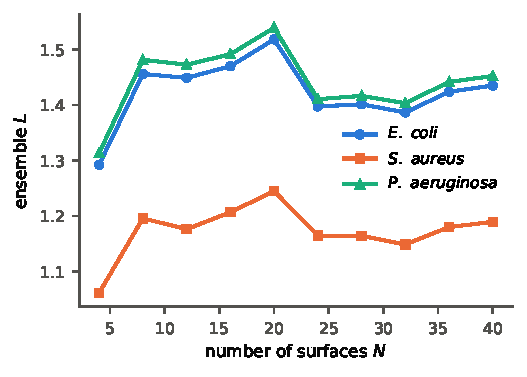
\includegraphics[width=0.55\linewidth]{figS1_running.pdf}
\caption{Ensemble $L=-\log_{10}\bar Y$ as reconstructions are added in a fixed order. The two halves of the ensemble give $L$ of \HalfEc{} (\Ec), \HalfSa{} (\Sa) and \HalfPa{} (\Pa).}
\label{fig:running}
\end{figure}

\clearpage
\section{Numerical verification}
\begin{table}[!ht]
\centering\small
\setlength{\tabcolsep}{5pt}
\renewcommand{\arraystretch}{1.05}
\caption{Grid refinement. Entries are $L=-\log_{10}Y$ for the nominal blade array (0), three draws from the prior (1--3) and the Sharklet AF-type cell. For the four blade arrays, the maximum $|\Delta L|$ between $\Delta x=0.10$ and \SI{0.07}{\micrometre} is \NumMax{} (mean \NumMean{}); the Sharklet cell changes by at most \NumShark{}. Halving or doubling the state time step changes $L$ by at most \NumTime{}.}\label{tab:numerics}
\begin{tabular}{llccccc}
\toprule Geometry & Species & \multicolumn{5}{c}{$\Delta x$ (\si{\micrometre})}\\
 & & 0.30 & 0.20 & 0.15 & 0.10 & 0.07\\\midrule
0 & \textit{E.~coli} & 1.15 & 1.26 & 1.30 & 1.28 & 1.30\\
0 & \textit{P.~aeruginosa} & 1.21 & 1.27 & 1.20 & 1.30 & 1.27\\
0 & \textit{S.~aureus} & 0.86 & 0.94 & 0.99 & 1.01 & 1.03\\
1 & \textit{E.~coli} & 1.71 & 1.87 & 1.94 & 1.93 & 1.95\\
1 & \textit{P.~aeruginosa} & 1.78 & 1.85 & 1.78 & 1.94 & 1.88\\
1 & \textit{S.~aureus} & 1.32 & 1.44 & 1.52 & 1.56 & 1.58\\
2 & \textit{E.~coli} & 0.90 & 0.99 & 1.02 & 1.02 & 1.04\\
2 & \textit{P.~aeruginosa} & 0.91 & 0.96 & 0.95 & 1.01 & 1.00\\
2 & \textit{S.~aureus} & 0.74 & 0.81 & 0.85 & 0.86 & 0.88\\
3 & \textit{E.~coli} & 1.67 & 1.85 & 1.89 & 1.88 & 1.90\\
3 & \textit{P.~aeruginosa} & 1.77 & 1.86 & 1.78 & 1.91 & 1.87\\
3 & \textit{S.~aureus} & 1.25 & 1.38 & 1.44 & 1.47 & 1.50\\
Sharklet & \textit{E.~coli} & 1.34 & 1.55 & 1.58 & 1.53 & 1.51\\
Sharklet & \textit{S.~aureus} & 1.02 & 1.16 & 1.23 & 1.29 & 1.29\\
Sharklet & \textit{P.~aeruginosa} & 1.39 & 1.59 & 1.36 & 1.58 & 1.43\\
\bottomrule
\end{tabular}
\end{table}


\section{Sensitivity analyses}
\begin{table}[h]\centering\small
\caption{Total-order Sobol indices of $L$ with respect to blade-array geometry (Saltelli design, $n=64$ base samples, 832 geometries, $\Delta x=\SI{0.2}{\micrometre}$, common lattice and roughness seeds; 95\% bootstrap intervals). Each input was sampled uniformly over the bounded support in table~\ref{tab:prior}; the indices quantify sensitivity under this design-space distribution. The production ensemble propagates the parameter-specific priors in table~\ref{tab:prior}, including truncated-normal distributions for the measured spacings and length.}\label{tab:sobolgeom}
\begin{tabular}{lccc}\toprule Parameter & \textit{E.~coli} & \textit{S.~aureus} & \textit{P.~aeruginosa}\\\midrule
pitch a & 0.794 [0.582, 1.012] & 0.818 [0.603, 1.044] & 0.773 [0.554, 0.977]\\
tip height & 0.200 [0.109, 0.314] & 0.177 [0.089, 0.280] & 0.225 [0.126, 0.358]\\
base width & 0.068 [0.040, 0.102] & 0.081 [0.045, 0.134] & 0.067 [0.040, 0.098]\\
pit depth & 0.041 [0.012, 0.079] & 0.031 [0.008, 0.061] & 0.051 [0.015, 0.099]\\
rough amp & 0.032 [0.018, 0.055] & 0.039 [0.021, 0.068] & 0.027 [0.014, 0.046]\\
pitch f & 0.023 [0.004, 0.059] & 0.029 [0.005, 0.080] & 0.023 [0.004, 0.059]\\
taper & 0.016 [0.010, 0.022] & 0.018 [0.010, 0.027] & 0.016 [0.011, 0.024]\\
length & 0.005 [0.003, 0.009] & 0.006 [0.003, 0.009] & 0.006 [0.003, 0.010]\\
pit b & 0.005 [0.002, 0.008] & 0.003 [0.002, 0.006] & 0.006 [0.003, 0.010]\\
jitter & 0.004 [0.001, 0.008] & 0.005 [0.002, 0.010] & 0.003 [0.001, 0.007]\\
pit a & 0.002 [0.001, 0.004] & 0.001 [0.000, 0.002] & 0.002 [0.001, 0.004]\\
\bottomrule\end{tabular}\end{table}

\begin{table}[h]\centering\small
\caption{Total-order Sobol indices with respect to mechanistic coefficients on the nominal blade array. Each multiplier is log-uniform on $[1/2,2]$ and scales the coefficient for all three species ($n=64$ base samples, 896 coefficient sets, $\Delta x=\SI{0.2}{\micrometre}$). First-order estimates were unstable at this sample size and are not reported. ``Contrast'' is $L_{Sa}/L_{Ec}$.}\label{tab:sobolmech}
\begin{tabular}{lcccc}\toprule Multiplier & $L$ \textit{E.~coli} & $L$ \textit{S.~aureus} & $L$ \textit{P.~aeruginosa} & contrast\\\midrule
beta & 0.301 & 0.306 & 0.301 & 0.056\\
body adhesion & 0.179 & 0.229 & 0.155 & 0.239\\
adhesion range & 0.167 & 0.203 & 0.145 & 0.166\\
transport penalty & 0.131 & 0.047 & 0.175 & 0.514\\
anchor rate & 0.044 & 0.038 & 0.048 & 0.002\\
capture rate & 0.019 & 0.010 & 0.025 & 0.033\\
compliance & 0.019 & 0.012 & 0.019 & 0.011\\
slope penalty & 0.006 & 0.004 & 0.008 & 0.002\\
detach rate & 0.002 & 0.001 & 0.002 & 0.001\\
appendage & 0.000 & 0.000 & 0.002 & 0.005\\
eps kinetics & 0.000 & 0.000 & 0.000 & 0.000\\
steric penalty & 0.000 & 0.000 & 0.000 & 0.000\\
\bottomrule\end{tabular}\end{table}

\begin{table}[h]\centering\small
\caption{Sensitivity of $L$ to a material difference between patterned surface and control. The control is simulated with body adhesion $\gamma_b$ scaled by $f$ while propensities on both surfaces are referenced to the unscaled flat energy (8 ensemble geometries, $\Delta x=\SI{0.15}{\micrometre}$).}\label{tab:chem}
\begin{tabular}{lccccc}\toprule Species & $f=0.8$ & 0.9 & 1.0 & 1.1 & 1.25\\\midrule
\textit{E.~coli} & 1.19 & 1.34 & 1.47 & 1.48 & 1.48\\
\textit{S.~aureus} & 0.83 & 1.02 & 1.18 & 1.25 & 1.25\\
\textit{P.~aeruginosa} & 1.17 & 1.29 & 1.39 & 1.40 & 1.40\\
\bottomrule\end{tabular}\end{table}


\FloatBarrier
\section{Arrival formulation and structural sensitivity}
The spatial arrival field $J$ in the primary model enters the free-cell supply and the coefficient for capture of transient cells. Let $i$ specify whether $J$ enters capture and $j$ specify whether it enters supply. We compared
\begin{align}
r_{FT}^{(i)}&=k_{\mathrm{cap}}J^i(0.55+0.45\bar p), &F_{\mathrm{target}}^{(j)}&=\lambda_{\mathrm{arr}}J^j,\\
(i,j)&=(1,1)\quad\text{dual pathway},&(i,j)&=(0,1)\quad\text{supply only},\qquad (1,0)\quad\text{capture only}.
\end{align}
The free-cell field was initialized to $F_{\mathrm{target}}^{(j)}$ in all three cases. At initialization, with nearly all sites available, the capture flux is proportional to $J^{i+j}$. The same reconstructed height field, species coefficients, contact field, EPS dynamics, numerical solver and mode-specific matched flat reference were used at every setting. The comparison used 40 identical geometric reconstructions at $\Delta x=\SI{0.10}{\micrometre}$. Bootstrap intervals were calculated by resampling reconstructed surfaces with replacement 10,000 times. The structural alternatives isolate the two appearances of the same $J$ field.

\begin{table}[htbp]\centering\small
\caption{Production-grid sensitivity to the representation of arrival. Values are ensemble log reductions with geometric-bootstrap 95\% intervals, and the ratio of \Sa{} to \Ec{} log reductions.}
\label{tab:structural}
\begin{tabular}{lcccc}\toprule
Model & \Ec{} $L$ & \Sa{} $L$ & \Pa{} $L$ & $L_{Sa}/L_{Ec}$\\\midrule
Both pathways & 1.43 (1.30--1.60) & 1.19 (1.08--1.32) & 1.45 (1.31--1.63) & 0.83\\
Supply only & 1.24 (1.12--1.38) & 1.09 (0.98--1.21) & 1.23 (1.11--1.37) & 0.88\\
Capture only & 1.16 (1.05--1.29) & 1.06 (0.96--1.17) & 1.14 (1.03--1.27) & 0.91\\
\bottomrule\end{tabular}
\end{table}


\FloatBarrier
\section{Lateral-spacing contrast and independent species parameters}
We varied adjacent-tip spacing between 3.4 and \SI{5.9}{\micrometre} in six steps at tip height \SI{1.5}{\micrometre}, using four common pairs of lattice and roughness seeds for each arrival formulation. In a separate coefficient experiment, 160 geometries were generated with seed 20261120. For every geometry, nine coefficients---body adhesion, adhesion range, transport slope and relief penalties, steric cost, appendage strength, detachment, anchoring and EPS activation---were multiplied by independently sampled uniform factors from $[0.8,1.2]$ for each species; $\beta$ and the relative body adhesion of the flat control received additional factors from the same interval, also drawn separately for each species. Each species was simulated against its matched flat control at $\Delta x=\SI{0.15}{\micrometre}$. Scenario quantiles describe the declared ranges and carry no fitted uncertainty.

\begin{table}[htbp]\centering\small
\caption{Lateral-packing contrasts in model log reduction, $L(3.4\,\si{\micrometre})-L(5.9\,\si{\micrometre})$, from the mean remaining fraction over four common lattice seeds. Positive values indicate stronger suppression for closer packing.}
\label{tab:spacing}
\begin{tabular}{lccc}\toprule
Model & \Ec{} & \Sa{} & \Pa{}\\\midrule
Both pathways & 1.94 & 1.69 & 1.89\\
Supply only & 1.56 & 1.44 & 1.49\\
Capture only & 1.50 & 1.40 & 1.43\\
\bottomrule\end{tabular}
\end{table}


\begin{figure}[htbp]\centering
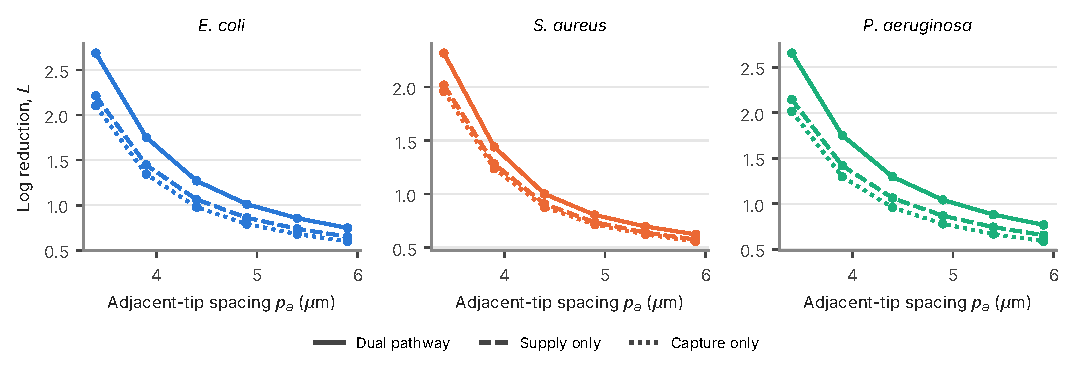
\includegraphics[width=\linewidth]{figS2_spacing.pdf}
\caption{Six-point lateral-packing sweep under the dual-pathway arrival formulation and the supply-only and capture-only alternatives. Each curve shows $-\log_{10}$ of the mean remaining fraction over four independently seeded surfaces at each spacing.}
\label{fig:spacingnew}\end{figure}

\begin{table}[htbp]\centering\small
\caption{Joint sensitivity scenarios with species-specific multipliers ($N=160$). Quantiles describe the distribution of prescribed model scenarios. The predicted \Pa{} 48~h reduction refits the shared endpoint exponent in each scenario.}
\label{tab:independent}
\begin{tabular}{lc}\toprule
Model diagnostic & Value\\\midrule
Nominal species ranking, \Ec{} suppression $>$ \Sa{} & 148/160 (92.5\%)\\
$L_{Sa}/L_{Ec}$, 5th--95th percentile & 0.55--1.02\\
\Ec{} model $L$, 5th--95th percentile & 0.84--2.83\\
\Sa{} model $L$, 5th--95th percentile & 0.61--2.29\\
\Pa{} mapped 48~h LR, 5th--95th percentile & 0.66--1.06\\
\bottomrule\end{tabular}
\end{table}


\FloatBarrier
\section{Small-sample uncertainty in the published contrast}
The ratio of published mean scale CFU to polystyrene CFU was transformed by $\mathrm{LR}=-\log_{10}(\bar r)$. We used the reported standard deviations for three biological replicates with the delta-method standard error $\mathrm{SE}(\mathrm{LR})\simeq\mathrm{SD}(r)/(\bar r\ln(10)\sqrt3)$. The Welch calculation treats the two transformed summary statistics as independent. Original replicate counts, within-pair correlations and the full observation distribution were unavailable, so the approximate $t$ intervals and test serve as small-sample diagnostics.

\begin{table}[htbp]\centering\small
\caption{Exploratory uncertainty diagnostic calculated from published summary statistics ($n=3$ biological replicates per species).}
\label{tab:smalln}
\begin{tabular}{lc}\toprule
Statistic & Value\\\midrule
\Ec{} log reduction, approximate 95\% $t$ interval & 0.81--1.05\\
\Sa{} log reduction, approximate 95\% $t$ interval & 0.25--1.05\\
Between-species difference (\Ec{} minus \Sa{}) & 0.28\\
Welch degrees of freedom & 2.35\\
Exploratory two-sided $p$ & 0.085\\
\bottomrule\end{tabular}
\end{table}

\FloatBarrier
\section{Geometric identifiability controls}
Four experiments separated the effect of adjacent-tip spacing from correlated changes in projected blade coverage, unmeasured three-dimensional relief and the arrangement of features at fixed density. Source code, per-configuration geometric descriptors and retention predictions are archived in Zenodo with the model code. Contrasts refer to the model observable $L=-\log_{10}(B_{\mathrm{pattern}}/B_{\mathrm{flat}})$ at model time $t=4.5$, and seed ranges describe geometric variation within the model.

\subsection{Projected-coverage-matched spacing designs}
Three adjacent-tip spacings ($p_a=3.8$, 4.4 and \SI{5.2}{\micrometre}) were evaluated on each of eight independently seeded lattices with identical seeds at every spacing. For the pit-bearing array, blade-base width was adjusted by binary search within the prior range $[1.6,3.4]$~\si{\micrometre} until the grid fraction of the projected blade mask was 0.35. A separate pit-free control set $d_p=0$ and matched its projected blade fraction to 0.46. These two fractional coverage targets were chosen because their respective intersections of feasible coverage ranges contained all three spacings without extrapolating the base-width prior. Consequently, direct differences between the pit-bearing and pit-free estimates also reflect the different target coverages. Each array was evaluated under the dual-pathway, supply-only and capture-only arrival models on the production grid $\Delta x=\SI{0.10}{\micrometre}$. The blade-mask coverage objective was independent of bacterial response, and each pairwise $L$ contrast used the same lattice and roughness seeds.

\begin{table}[htbp]\centering\scriptsize
\caption{Paired log-reduction contrast at matched projected blade coverage, $\Delta L=L(p_a=3.8\,\si{\micrometre})-L(p_a=5.2\,\si{\micrometre})$. Entries are mean [minimum, maximum] over eight common surface seeds, with blade-base width adjusted within its prior range. Pit-bearing and pit-free arrays use target coverages of 0.35 and 0.46, respectively.}
\label{tab:geomcov}
\begin{tabular}{llccc}\toprule
Pit condition & Arrival formulation & \Ec{} & \Sa{} & \Pa{}\\\midrule
Pits present & Both pathways & +0.71 [+0.69, +0.72] & +0.59 [+0.57, +0.59] & +0.68 [+0.65, +0.69]\\
Pits present & Supply only & +0.55 [+0.53, +0.55] & +0.49 [+0.48, +0.50] & +0.51 [+0.49, +0.52]\\
Pits present & Capture only & +0.51 [+0.49, +0.52] & +0.46 [+0.45, +0.47] & +0.47 [+0.46, +0.48]\\
Pits absent & Both pathways & +0.48 [+0.45, +0.49] & +0.53 [+0.51, +0.54] & +0.43 [+0.41, +0.45]\\
Pits absent & Supply only & +0.37 [+0.35, +0.39] & +0.46 [+0.44, +0.47] & +0.33 [+0.32, +0.35]\\
Pits absent & Capture only & +0.35 [+0.33, +0.36] & +0.44 [+0.42, +0.45] & +0.31 [+0.29, +0.32]\\
\bottomrule\end{tabular}
\end{table}


\begin{figure}[htbp]\centering
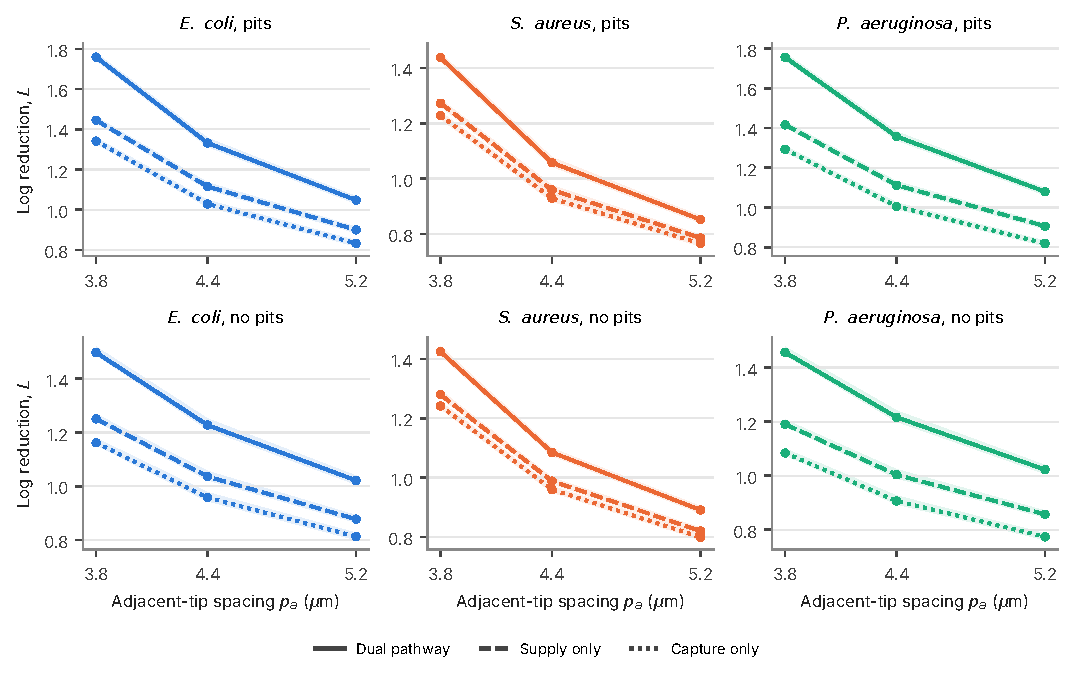
\includegraphics[width=\linewidth]{figS3_matched_coverage.pdf}
\caption{Model log reductions over the matched-coverage lateral-spacing design. The first row contains arrays with pits and the second row contains pit-free arrays. Solid, dashed and dotted curves correspond to the dual-pathway, supply-only and capture-only arrival formulations; shaded regions represent one standard deviation across eight reconstructed textures. The two pit conditions have distinct coverage targets and should be interpreted within condition.}
\label{fig:coveragecontrols}
\end{figure}

\subsection{Variation in unmeasured blade height and pit depth}
The factorial experiment combined $p_a\in\{3.8,4.4,5.0\}$~\si{\micrometre}, tip height $h_t\in\{0.5,1.5,3.0\}$~\si{\micrometre} and pit depth $d_p\in\{0.5,2.5\}$~\si{\micrometre}. Eight nuisance-geometry draws sampled the measured following pitch and blade length from their truncated-normal priors and the blade width, taper, pit size, jitter and roughness from the bounded priors reported in table~\ref{tab:prior}. Each nuisance draw was reused across all eighteen factorial combinations, yielding 144 distinct patterned surfaces and 432 species-model predictions under the dual-pathway arrival model at $\Delta x=\SI{0.10}{\micrometre}$. Paired contrasts compare close and widely spaced blades for the same nuisance geometry, height and pit depth. The 48 pairwise contrasts per species share eight nuisance draws.

\begin{table}[htbp]\centering\small
\caption{Effect of lateral pitch across unmeasured relief in the dual-pathway model. Paired $\Delta L=L(3.8)-L(5.0)$ is calculated for eight nuisance-geometry draws at each tip height and pit depth. Entries are mean [range] over the sixteen combinations of draw and pit depth at each height.}
\label{tab:geom3d}
\begin{tabular}{llccc}\toprule
Species & Tip height (\si{\micrometre}) & Mean $\Delta L$ [range] & Positive & Draws\\\midrule
\Ec{} & 0.5 & +0.39 [+0.18, +0.69] & 16 / 16 & 8\\
\Ec{} & 1.5 & +0.79 [+0.38, +1.48] & 16 / 16 & 8\\
\Ec{} & 3.0 & +1.22 [+0.57, +2.49] & 16 / 16 & 8\\
\addlinespace
\Sa{} & 0.5 & +0.32 [+0.15, +0.58] & 16 / 16 & 8\\
\Sa{} & 1.5 & +0.66 [+0.30, +1.27] & 16 / 16 & 8\\
\Sa{} & 3.0 & +1.01 [+0.44, +2.07] & 16 / 16 & 8\\
\addlinespace
\Pa{} & 0.5 & +0.37 [+0.17, +0.65] & 16 / 16 & 8\\
\Pa{} & 1.5 & +0.76 [+0.36, +1.44] & 16 / 16 & 8\\
\Pa{} & 3.0 & +1.20 [+0.55, +2.48] & 16 / 16 & 8\\
\bottomrule\end{tabular}
\end{table}


\begin{figure}[htbp]\centering
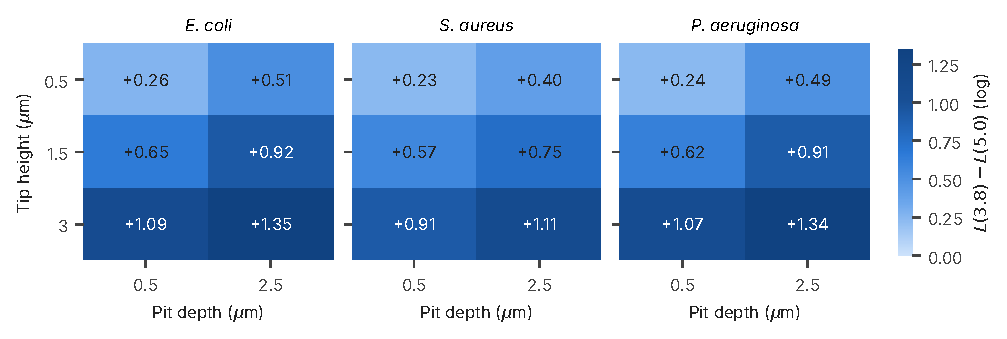
\includegraphics[width=.94\linewidth]{figS4_factorial_3d.pdf}
\caption{Mean paired log-reduction difference $L(3.8)-L(5.0)$ as a function of the unmeasured tip height and pit depth in the primary dual-pathway model. Each cell averages eight matched nuisance-geometry draws with the other geometric parameters sampled from their declared priors.}
\label{fig:factorialcontrols}
\end{figure}

\subsection{Arrangement at fixed feature density}
We altered the offset of alternating rows by $\delta\in\{0,0.25,0.5\}$, measured in units of the following-blade pitch. The $\delta=0.5$ configuration is the staggered reconstruction used throughout. For all three phases, the perpendicular separation between rows, following pitch, number of blade features, nominal blade geometry and pit dimensions were held fixed. The model predictions were computed for eight matched seeds in both the intact-pit and pit-free versions, using the primary arrival formulation and $\Delta x=\SI{0.10}{\micrometre}$. Density is thus fixed exactly, whereas the diagonal distance between neighbouring tips changes with row phase. Differences in projected blade-mask fraction are reported in the source CSV for each configuration.

\begin{table}[htbp]\centering\small
\caption{Fixed-density row-arrangement contrast, $L(\delta=0.5)-L(\delta=0)$, in units of $10^{-3}$ log; $\delta$ is the offset of alternating rows in units of the following pitch. Entries are mean [minimum, maximum] across eight common surface seeds. Blade count, column separation, pitch and blade dimensions are fixed. Results use the dual-pathway formulation.}
\label{tab:geomphase}
\begin{tabular}{llcc}\toprule
Pit condition & Species & $\Delta L$ [range] & Positive pairs\\\midrule
Pits present & \Ec{} & +0.4 [\ensuremath{-}9.2, +4.2] & 4 / 8\\
Pits present & \Sa{} & +1.3 [\ensuremath{-}1.9, +4.1] & 6 / 8\\
Pits present & \Pa{} & \ensuremath{-}0.9 [\ensuremath{-}10.9, +2.8] & 4 / 8\\
Pits absent & \Ec{} & \ensuremath{-}0.1 [\ensuremath{-}7.9, +3.3] & 5 / 8\\
Pits absent & \Sa{} & +0.7 [\ensuremath{-}2.5, +3.3] & 5 / 8\\
Pits absent & \Pa{} & \ensuremath{-}0.3 [\ensuremath{-}7.6, +3.2] & 4 / 8\\
\bottomrule\end{tabular}
\end{table}


\begin{figure}[htbp]\centering
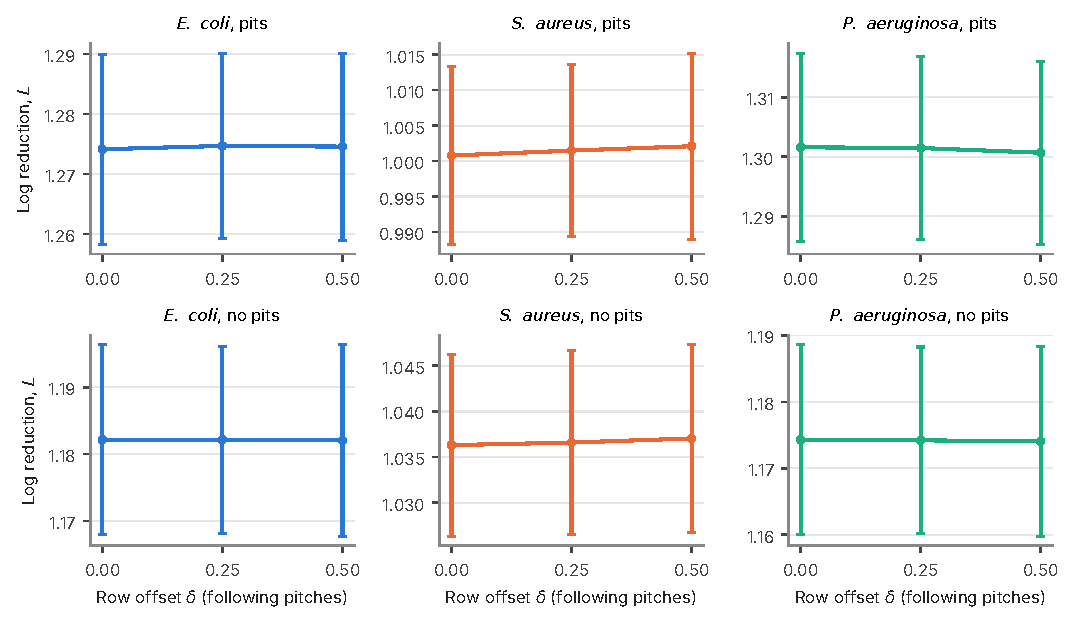
\includegraphics[width=\linewidth]{figS5_fixed_density_phase.pdf}
\caption{Fixed-density row-phase response. Each curve is the mean $L$ across eight common lattice seeds for the primary arrival formulation; error bars show one standard deviation between seeds. The upper row lacks pits and the lower row retains the nominal pits. The phase parameter changes the lateral arrangement at fixed feature count and row separation.}
\label{fig:phasecontrols}
\end{figure}

\subsection{Grid sensitivity near narrow channels}
The original numerical test included a typical array and three prior draws. The additional experiment examines a close-packed nominal array ($p_a=3.4$~\si{\micrometre}, $w_0=2.2$~\si{\micrometre}), a tall and crowded close-packed array ($h_t=3.0$~\si{\micrometre}, $w_0=3.2$~\si{\micrometre}), a low and narrow close-packed array ($h_t=0.5$~\si{\micrometre}, $w_0=1.6$~\si{\micrometre}), and a wide-spacing nominal reference ($p_a=5.9$~\si{\micrometre}). Each geometry and species was simulated at $\Delta x=0.15$, 0.10 and \SI{0.07}{\micrometre} in the primary arrival formulation. Differences between the two finest grids are empirical convergence diagnostics at these resolutions, with no extrapolation to the continuum limit. Because the closest and most crowded cases had larger grid effects, we also ran them at $\Delta x=\SI{0.05}{\micrometre}$. The further differences, reaching \GeomExtremeMaxAdditional{} log units, show that extreme high-relief point predictions remain numerically sensitive.

\begin{table}[htbp]\centering\small
\caption{Grid checks in close-packed and comparison geometries (dual-pathway model). The last column is the signed difference between the production grid and the first refinement; the \SI{0.05}{\micrometre} extension was run for the two close-packed geometries with the largest differences.}
\label{tab:geomgrid}
\begin{tabular}{llccccc}\toprule
Geometry & Species & $L_{0.15}$ & $L_{0.10}$ & $L_{0.07}$ & $L_{0.05}$ & $L_{0.10}-L_{0.07}$\\\midrule
Close, nominal & \Ec{} & 2.767 & 2.680 & 2.753 & 2.831 & \ensuremath{-}0.073\\
Close, nominal & \Sa{} & 2.263 & 2.311 & 2.368 & 2.386 & \ensuremath{-}0.057\\
Close, nominal & \Pa{} & 2.363 & 2.650 & 2.534 & 2.669 & +0.116\\
\addlinespace
Close, crowded/tall & \Ec{} & 4.435 & 4.358 & 4.452 & 4.555 & \ensuremath{-}0.094\\
Close, crowded/tall & \Sa{} & 3.502 & 3.563 & 3.640 & 3.665 & \ensuremath{-}0.077\\
Close, crowded/tall & \Pa{} & 4.041 & 4.449 & 4.301 & 4.484 & +0.148\\
\addlinespace
Close, short/narrow & \Ec{} & 1.449 & 1.412 & 1.447 & -- & \ensuremath{-}0.034\\
Close, short/narrow & \Sa{} & 1.197 & 1.208 & 1.245 & -- & \ensuremath{-}0.037\\
Close, short/narrow & \Pa{} & 1.259 & 1.366 & 1.333 & -- & +0.033\\
\addlinespace
Wide, nominal & \Ec{} & 0.759 & 0.751 & 0.760 & -- & \ensuremath{-}0.009\\
Wide, nominal & \Sa{} & 0.621 & 0.627 & 0.639 & -- & \ensuremath{-}0.012\\
Wide, nominal & \Pa{} & 0.729 & 0.770 & 0.759 & -- & +0.012\\
\bottomrule\end{tabular}
\end{table}


\begin{figure}[htbp]\centering
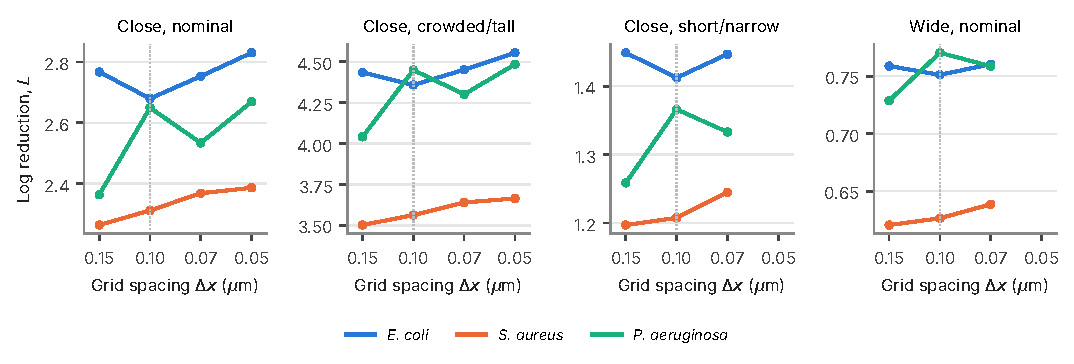
\includegraphics[width=.92\linewidth]{figS6_close_grid.pdf}
\caption{Signed log-reduction difference between grid spacings of 0.10 and \SI{0.07}{\micrometre} for each geometric test case and species. The absolute value measures sensitivity to refinement in the tested interval.}
\label{fig:gridcontrols}
\end{figure}
\FloatBarrier


\subsection{Finer-grid replication of the primary coverage-matched contrast}
For four of the eight paired texture seeds (11, 22, 33 and 44), each pit-bearing and pit-free array at $p_a=3.8$ and \SI{5.2}{\micrometre} was recalculated at $\Delta x=\SI{0.07}{\micrometre}$. The blade-base widths remained fixed at their values selected from the projected-coverage objective at $\Delta x=\SI{0.10}{\micrometre}$; this is a direct numerical refinement of the same reconstructed surfaces, without recalibrating the geometry or using the bacterial predictions during matching. Every one of the \GeomFinePos{} paired refined log-reduction differences was positive, and the largest absolute change in the paired difference between the two grid spacings was \GeomFineMaxDeltaError{} log units. The distinction between a stable contrast and numerically sensitive high-relief point estimates is retained in the main conclusions.

\begin{table}[htbp]\centering\small
\caption{Finer-grid repetition of the coverage-matched contrast, $\Delta L=L(3.8)-L(5.2)$. Widths were fixed at the values selected on the \SI{0.10}{\micrometre} grid and the same surfaces were re-evaluated at \SI{0.07}{\micrometre}. Entries are mean paired contrasts across four matched seeds, the largest absolute change in any paired contrast between resolutions, and the count of positive refined contrasts.}
\label{tab:geomfine}
\begin{tabular}{llcccc}\toprule
Pits & Species & Mean $\Delta L_{0.10}$ & Mean $\Delta L_{0.07}$ & Max $|\delta(\Delta L)|$ & Positive\\\midrule
Pits present & \Ec{} & +0.706 & +0.731 & 0.028 & 4/4\\
Pits present & \Sa{} & +0.582 & +0.597 & 0.016 & 4/4\\
Pits present & \Pa{} & +0.672 & +0.619 & 0.056 & 4/4\\
Pits absent & \Ec{} & +0.472 & +0.492 & 0.024 & 4/4\\
Pits absent & \Sa{} & +0.531 & +0.515 & 0.017 & 4/4\\
Pits absent & \Pa{} & +0.430 & +0.385 & 0.047 & 4/4\\
\bottomrule\end{tabular}
\end{table}


\begin{figure}[htbp]\centering
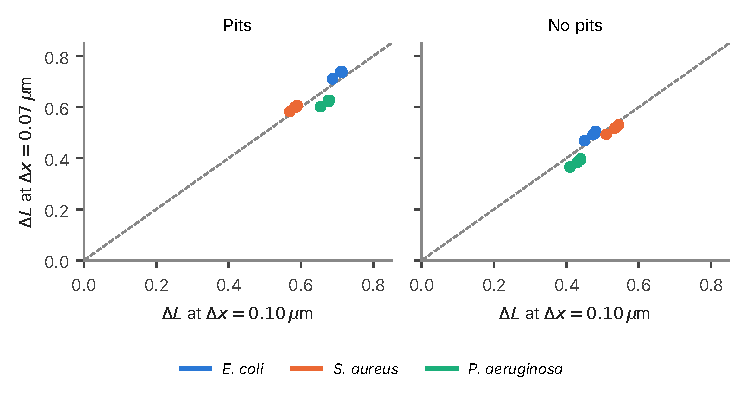
\includegraphics[width=.9\linewidth]{figS7_matched_grid.pdf}
\caption{Direct numerical refinement of the matched-coverage design. Each point gives a paired log-reduction contrast $L(3.8)-L(5.2)$ for one species, one pit treatment and one of four matched texture seeds. The dashed line indicates equality between calculations at $\Delta x=0.10$ and \SI{0.07}{\micrometre}. All 24 refined contrasts are positive.}
\label{fig:matchedgrid}
\end{figure}

\FloatBarrier
\bibliographystyle{unsrtnat}
\bibliography{refs}
\end{document}
